\subsection{Integral elements over a ring}

THEOREM 1. Let A be a (commutative) ring, R an algebra over A (not necessarily commutative) and x an element of R. The following properties are equivalent:

(E \(_{I}\) ) x is a root of a monic polynomial in the polynomial ring A{[}X{]}.

\((\mathbf{E}_{\mathrm{II}})\) The subalgebra \(\mathbf{A}[x]\) of \(\mathbf{R}\) is a finitely generated A-module.

\((E_{\mathrm{III}})\) There exists a faithful module over the ring A{[}x{]} which is a finitely generated A-module.

Let us show first that \((\mathbf{E}_{\mathbf{I}})\) implies \((\mathbf{E}_{\mathbf{II}})\) . Let

\[
\mathrm{X} ^ {n} + a _ {1} \mathrm{X} ^ {n - 1} + \dots + a _ {n}
\]

be a monic polynomial in A{[}X{]} with x as a root; for every integer \(q \geqslant 0\) let \(M_{q}\) be the sub-A-module of R generated by 1, \(x, \ldots, x^{n+q}\) . Then

\[
x ^ {n + q} = - a _ {1} x ^ {n + q - 1} - \dots - a _ {n} x ^ {q} \in \mathrm{M} _ {q - 1}
\]

for all \(q \geqslant 1\) , whence, by induction on \(q\) ,

\[
\mathbf {M} _ {q} = \mathbf {M} _ {q - 1} = \dots = \mathbf {M} _ {0}.
\]

We conclude that A{[}x{]} is equal to \(M_{0}\) and is therefore a finitely generated A-module.

As the commutative ring A{[}x{]} is a faithful module over itself, \((\mathbf{E}_{\mathrm{II}})\) implies \((\mathbf{E}_{\mathrm{III}})\) .

Finally, the fact that \((\mathbf{E}_{\mathrm{III}})\) implies \((\mathbf{E}_{\mathrm{I}})\) will follow from the following more precise lemma:

LEMMA 1. Let A be a ring, R an algebra (not necessarily commutative) over A and x an element of R. Let M be a faithful module over A{[}x{]} which is a finitely generated A-module. If q is an ideal of A such that xM ⊂ qM, then x is a root of a monic polynomial with coefficients in A all of whose coefficients other than the dominant coefficient belong to q.

Let \((u_{i})_{1\leqslant i\leqslant n}\) be a finite family of elements of M such that \(\mathbf{M} = \sum_{i = 1}^{n}\mathbf{A}u_{i}\) . For all \(i\) , there exists by hypothesis a finite family \((q_{ij})_{1\leqslant j\leqslant n}\) of elements of q such that

\[
x u _ {i} = \sum_ {j = 1} ^ {n} q _ {i j} u _ {j} \quad \text { for } \quad 1 \leqslant i \leqslant n.
\]

Therefore (Algebra, Chapter III, § 8) if \(d\) is the determinant of the matrix \((q_{ij} - \delta_{ij}x)\) with elements in A{[}x{]} ( \(\delta_{ij}\) denoting the Kronecker index), then \(du_i = 0\) for all \(i\) and hence \(d\mathbf{M} = 0\) ; as M is assumed to be a faithful A{[}x{]}-module, necessarily \(d = 0\) . This means that \(x\) is a root of the polynomial \(\det(q_{ij} - \delta_{ij}\mathbf{X})\) in A{[}X{]} which, up to a sign, is a monic polynomial whose coefficients other than the dominant coefficient belong to q.

DEFINITION 1. Let A be a ring and R an A-algebra (not necessarily commutative). An element \(x \in \mathbb{R}\) is called integral over \(A\) if it satisfies the equivalent properties \((\mathrm{E}_{\mathrm{I}}), (\mathrm{E}_{\mathrm{II}}), (\mathrm{E}_{\mathrm{III}})\) of Theorem 1.

A relation of the form \(\mathrm{P}(x)=0\) , where P is a monic polynomial in A{[}X{]} is also called an equation of integral dependence with coefficients in A.

\textbf{Examples}\par

\begin{enumerate}
\def\labelenumi{(\arabic{enumi})}
\tightlist
\item
  Let K be a (commutative) field and R a K-algebra; to say that an element \(x \in R\) is integral over K is equivalent to saying that x is a root of a non-constant polynomial in the ring K{[}X{]}; generalizing the terminology introduced when R is an extension of K (Algebra, Chapter V, §3, no. 3), the elements \(x \in R\) which are integral over K are also called the algebraic elements of R over K.
\end{enumerate}

* (2) The elements of \(\mathbf{Q}(i)\) which are integral over \(\mathbf{Z}\) are the elements of the form \(a + ib\) where \(a \in \mathbf{Z}\) and \(b \in \mathbf{Z}\) (``Gaussian integers''); the elements of \(\mathbf{Q}(\sqrt{5})\) which are integral over \(\mathbf{Z}\) are the elements of the form \((a + b\sqrt{5})/2\) where \(a\) and \(b\) belong to \(\mathbf{Z}\) and are both even or both odd (for these two examples see Exercise 1).*

\begin{enumerate}
\def\labelenumi{(\arabic{enumi})}
\setcounter{enumi}{2}
\tightlist
\item
  The complex numbers integral over \(\mathbf{Z}\) are also called algebraic integers.
\end{enumerate}

\textbf{Remarks}\par

\begin{enumerate}
\def\labelenumi{(\arabic{enumi})}
\item
  Let A' be the subring of R (contained in the centre of R) the image of A under the ring homomorphism A → R which defines the A-algebra structure on R. Clearly it is equivalent to say that an element of R is integral over A or that it is integral over A'.
\item
  Let \(R'\) be a sub-A-algebra of R; the elements of \(R'\) which are integral over A are just the elements of R which are integral over A and belong to \(R'\) ; this often allows us not to specify the algebra to which an integral element over A belongs, when no confusion can arise.
\end{enumerate}

PROPOSITION 1. Let A be a ring, R an algebra over A (not necessarily commutative) and x an element of R. For x to be integral over A, it is necessary and sufficient that A{[}x{]} be contained in a subalgebra R' of R which is a finitely generated A-module.

The condition is obviously necessary by virtue of property \((\mathrm{E}_{\mathrm{II}})\) ; it is also sufficient by virtue of \((\mathrm{E}_{\mathrm{III}})\) , for \(R'\) is a faithful A{[}x{]}-module (since it contains the unit element of R).

COROLLARY. Let A be a Noetherian ring, R an A-algebra (not necessarily commutative) and x an element of R. For x to be integral over A, it is necessary and sufficient that there exist a finitely generated submodule of R containing A{[}x{]}.

The condition is necessary by virtue of \((\mathrm{E}_{\mathrm{II}})\) ; it is sufficient for if A{[}x{]} is a sub-A-module of a finitely generated A-module, it is itself a finitely generated A-module (Algebra, Chapter VIII, §2, no. 3, Proposition 7).

\pandocbounded{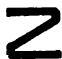
\includegraphics[keepaspectratio]{images/part002_1e1abfe7.jpg}}

The hypothesis that A is Noetherian cannot be omitted from the statement (Exercise 2).

DEFINITION 2. Let A be a ring. An A-algebra R (not necessarily commutative) is called integral over A if every element of R is integral over A. R is called finite over A if R is a finitely generated A-module.

It follows from Proposition 1 that every finite A-algebra is integral; if R is commutative and a finite A-algebra, R is obviously a finitely generated A-algebra; the converse is false.

Example (4) If M is a finitely generated A-module, the algebra \(\operatorname{End}_{\mathbf{A}}(\mathbf{M})\) of endomorphisms of M is integral over A by virtue of \((\mathrm{E}_{\mathrm{III}})\) ; in particular, for every integer n, the matrix algebra \(\mathbf{M}_{n}(\mathbf{A}) = \operatorname{End}_{\mathbf{A}}(\mathbf{A}^{n})\) is integral (and even finite) over A.

PROPOSITION 2. Let A, A' be two rings, R an A-algebra, R' an A'-algebra (not necessarily commutative) and \(f\colon\mathbf{A}\to\mathbf{A}'\) and \(g\colon\mathbf{R}\to\mathbf{R}'\) two ring homomorphisms such that the diagram

\pandocbounded{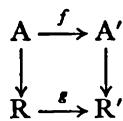
\includegraphics[keepaspectratio]{images/part002_4af46373.jpg}}

is commutative. If an element \(x \in R\) is integral over A, then \(g(x)\) is integral over \(A'\) . If \(x^{n} + a_{1}x^{n-1} + \cdots + a_{n} = 0\) where \(a_{i} \in A\) for \(1 \leqslant i \leqslant n\) , we deduce that

\[
(g (x)) ^ {n} + f \left(a _ {1}\right) (g (x)) ^ {n - 1} + \dots + f \left(a _ {n}\right) = 0.
\]

COROLLARY 1. Let A be a ring, B a (commutative) A-algebra and C a (not necessarily commutative) B-algebra. Then every element \(x \in \mathbf{C}\) which is integral over A is integral over B.

COROLLARY 2. Let K be a field, L an extension of K and x, \(x'\) two elements of L which are conjugate over K (Algebra, Chapter V, § 6, no. 2). If A is a subring of K and x is integral over A, \(x'\) is also integral over A.

There exists a K-isomorphism \(f\) of \(\mathbf{K}(x)\) onto \(\mathbf{K}(x')\) such that \(f(x) = x'\) and the elements of \(\mathbf{A}\) are invariant under \(f\) .

COROLLARY 3. Let A be a ring, B a (commutative) A-algebra and C a (not necessarily commutative) B-algebra. If C is integral over A, C is integral over B.

PROPOSITION 3. Let \((\mathbf{R}_i)_{1\leqslant i\leqslant n}\) be a finite family of (not necessarily commutative)

A-algebras and let \(\mathbf{R} = \prod_{i=1}^{n} \mathbf{R}_i\) be their product. For an element \(x = (x_i)_{1 \leq i \leq n}\) of \(\mathbf{R}\) to be integral over \(\mathbf{A}\) , it is necessary and sufficient that each of the \(x_i\) be integral over \(\mathbf{A}\) . For \(\mathbf{R}\) to be integral over \(\mathbf{A}\) , it is necessary and sufficient that each of the \(\mathbf{R}_i\) be integral over \(\mathbf{A}\) .

It is obviously sufficient to prove the first assertion. The condition is necessary by Proposition 2. Conversely, if each of the \(x_{i}\) is integral over \(A\) , the subalgebra \(A[x_{i}]\) of \(R_{i}\) is a finitely generated \(A\) -module and hence so is the subalgebra \(\prod_{i=1}^{n} \mathrm{A}[x_i]\) of R; as \(\mathrm{A}[x]\) is contained in this subalgebra, \(x\) is integral over A by Proposition 1.

PROPOSITION 4. Let A be a ring, R an A-algebra (not necessarily commutative) and \((x_{i})_{1\leq i\leq n}\) a finite family of elements of R which are pairwise permutable. If, for all \(i, x_{i}\) is integral over \(A[x_{1},\cdots,x_{i-1}]\) (and in particular if all the \(x_{i}\) are integral over A), then the subalgebra \(A[x_{1},\ldots,x_{n}]\) of R is a finitely generated A-module.

We argue by induction on \(n\) , the proposition being just \((\mathbf{E}_{\mathrm{II}})\) for \(n = 1\) . The induction hypothesis implies that \(B = A[x_{1}, \cdots, x_{n-1}]\) is a finitely generated A-module; as \(x_{n}\) is integral over B, \(B[x_{n}] = A[x_{1}, \cdots, x_{n}]\) is a finitely generated B-module and therefore also a finitely generated A-module (Algebra, Chapter II, § 1, no. 13, Proposition 25).

COROLLARY 1. Let A be a ring and R a (commutative) A-algebra. The set of elements of R integral over A is a subalgebra of R.

In fact, if x, y are two elements of R integral over A, it follows from Proposition 4 that A{[}x, y{]} is a finitely generated A-module; as it contains \(x + y\) and xy, the corollary follows from Proposition 1.

\pandocbounded{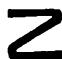
\includegraphics[keepaspectratio]{images/part002_90735efb.jpg}}

In a non-commutative algebra the sum and product of two integral elements over A are not necessarily integral over A (Exercise 4).

COROLLARY 2. Let A be a ring, R an A-algebra (not necessarily commutative) and E a set of elements of R which are pairwise permutable and integral over A. Then the sub-A-algebra B of R generated by E is integral over A.

Every element of B belongs to a sub-A-algebra of B generated by a finite subset of E.

Remark (3) It follows from Proposition 4 that every commutative A-algebra integral over A is the union of a right directed family of finite subalgebras over A.

PROPOSITION 5. Let A be a ring and A' and R two (commutative) A-algebras. If R is integral over A, \(R \otimes_{A} A'\) is integral over A'.

Consider any element \(x' = \sum_{i=1}^{n} x_i \otimes a_i'\) of \(\mathbf{R} \otimes_{\mathbf{A}} \mathbf{A}'\) , where the \(x_i\) belong to \(\mathbf{R}\) and the \(a_i'\) to \(\mathbf{A}'\) ; as \(x_i \otimes a_i' = (x_i \otimes 1)a_i'\) and the \(x_i \otimes 1\) are integral over \(\mathbf{A}'\) (Proposition 2), so is \(x\) .

COROLLARY. Let R be a ring and A, B, C subrings of R such that \(A \subset B\) . If B is integral over A, C{[}B{]} is integral over C{[}A{]}.

\(B \otimes_{A} C[A]\) is integral over \(C[A]\) by Proposition 5 and hence so is the canonical image \(C[B]\) of \(B \otimes_{A} C[A]\) in \(R\) (considered as an A-algebra) by Proposition 2.

PROPOSITION 6. Let A be a ring, B a (commutative) A-algebra and C a (not necessarily commutative) B-algebra. If B is integral over A and C is integral over B, then C is integral over A.

It is sufficient to verify that every \(x \in C\) is integral over A. By hypothesis there exists a monic polynomial \(X^{n} + b_{1}X^{n-1} + \cdots + b_{n}\) with coefficients in B with x as a root; then x is integral over \(B' = A[b_{1}, \ldots, b_{n}]\) and \(B'[x]\) is therefore a finitely generated \(B'\) -module. But as B is integral over A, \(B'\) is a finitely generated A-module (Proposition 4); we conclude that \(\mathbf{B}'[x]\) is also a finitely generated A-module (Algebra, Chapter II, §1, no. 13, Proposition 25) and therefore \(x\) is integral over \(\mathbf{A}\) .

COROLLARY. Let A be a ring and R, R' two (commutative) A-algebras integral over A. Then \(R \otimes_{A} R'\) is integral over A.

\(R \otimes_{A} R'\) is integral over \(R'\) (Proposition 5) and hence the conclusion follows from Proposition 6.

